\chapter{Fluxo em redes}

Capítulo 6 de Szwarcfiter, \textit{Grafos e Algoritmos Computacionais}~\cite{Szwarcfiter1986grafos}.

%%%%%%%%%%%%%%%%%%%%%%%%%%%%%%%%%%%%%%%%%%%%%%%%%%%%%%%%%%%%
\section{Introdução}

Serão vistos neste capítulo definições e algoritmos relacionados a fluxo em redes.

%%%%%%%%%%%%%%%%%%%%%%%%%%%%%%%%%%%%%%%%%%%%%%%%%%%%%%%%%%%%
\section{O problema do fluxo máximo}

% Página 22

\begin{easylist}

  & Multidigrafo $D(V,E)$ é um conjunto finito não vazio $V$ e um multiconjunto $E$ de pares ordenados de elementos distintos de $V$. Portanto, pode haver mais de uma aresta $(v, w)$ simultaneamente.

  & Rede é um multidigrafo $D(V, E)$ em que a cada aresta $e$ está associado uma capacidade $c(e)$.

  & Fluxo: considere uma rede $D(V, E)$ contendo dois vértices especiais $s, t \in V$ denominados origem e destino respectivamente. Os vértices $s$ e $t$ possuem as seguintes propriedades:

  && $s$ é uma fonte que alcança todos os vértices;
  && $t$ é um sumidouro alcançado por todos os vértices.

  Um fluxo $f$ de $s$ a $t$ em $D$ é uma função que, a cada aresta $e \in E$ associa um número real não negativo $f(e)$ com as seguintes propriedades:
  
  && $0 \leq f(e) \leq c(e)$
  && $\sum_{w_1} f(w_1, v) = \sum_{w_2} f(v, w_2)$ para todo $v \neq s, t$. 

  & Fluxo ilegal: fluxo que não satisfaz as propriedades da definição.

  & Valor do fluxo no vértice $v$ é dado pela somatória dos fluxos nas arestas convergentes a $v$ ou divergentes de $v$. De forma análoga, é dada pela soma dos fluxos das arestas divergentes de $s$ ou convergentes a $t$.

  & Valor do fluxo no digrafo $D(V, E)$ é denotado por $f(D)$ e é igual a $f(s)$.

  & Aresta saturada: é uma aresta em que $f(e) = c(e)$.

  & Vértice saturado: é um vértice com todas as arestas convergentes e/ou divergentes saturadas.

  & Fluxo maximal: fluxo onde todo caminho de $s$ a $t$ possui alguma aresta saturada.

  & Corte: seja $S \subseteq V$ um subconjunto de vértices tal que $s \in S$, $t \notin S$ e $\bar S = V - S$ seu complemento, um corte $(S, \bar S)$ em $D$ é o subconjunto das arestas que possuem uma extremidade em $S$ e outra em $\bar S$.

  & Capacidade de um corte $c(S, \bar S)$: sejam
  $(S, \bar S)^+ = \{(v, w) \in E | v \in S, w \in \bar S\}$ e
  $(S, \bar S)^- = \{(v, w) \in E | v \in \bar S, w \in S\}$, a capacidade $c(S, \bar S)$ é o somatório das capacidades das arestas de $(S, \bar S)^+$, ou seja,
  \[ c(S, \bar S) = \sum_{e \in (S, \bar S)^+} c(e) \].

  & Fluxo no corte $f(S, \bar S)$: seja $f$ um fluxo e $(S, \bar S)$ um corte, o fluxo $f(S, \bar S)$ no corte $(S, \bar S)$ é definido como a diferença 
  \[ f(S, \bar S) = \sum_{e \in (S, \bar S)^+} f(e) - \sum_{e \in (S, \bar S)^-} f(e) \].

  & Lema: seja $f$ um fluxo e $(S, \bar S)$ um corte em um digrafo $D$. Temos que $f(S, \bar S) = f(D)$.

  & Aresta direta: aresta $e$ tal que $c(e) - f(e) > 0$

  & Aresta contrária: aresta $e$ tal que $f(e) > 0$

  & Digrafo residual $D'(F)$: seja $D(V, E)$ um digrafo e $f$ um fluxo,
  && se $(v, w)$ é aresta direta de $D$ então $(v, w)$ é aresta direta de $D'$ com capacidade $c'(v, w) = c(v, w) - f(v, w)$.
  && se $(v, w)$ é aresta contrária de $D$ então $(w, v)$ é aresta contrária de $D'$ com capacidade $c'(w, v) = f(v, w)$.

\begin{figure}[t]
  \begin{center}
    \begin{tabular}{c}
      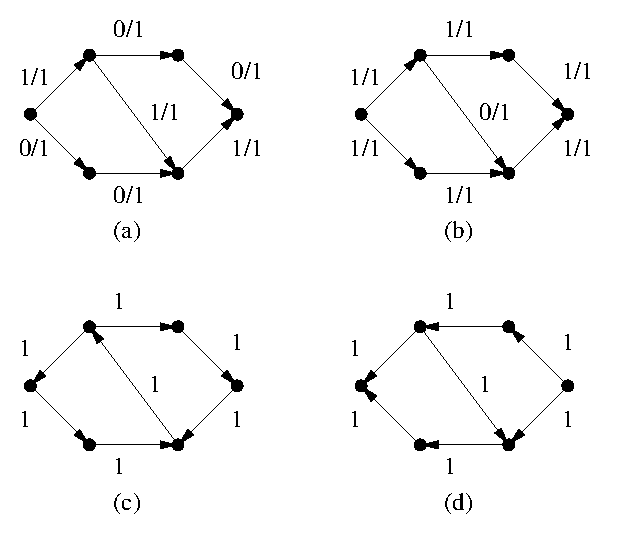
\includegraphics[width=0.7\textwidth]{images/06/flow01.eps}
    \end{tabular}
  \end{center}
  \caption{\label{fig:3:1} (a) Fluxo maximal; (b) fluxo máximo; (c) digrafo residual no fluxo maximal; (d) digrafo residual no fluxo máximo.}
  \source{Szwarcfiter~\cite{Szwarcfiter1986grafos}.}
\end{figure}

  & Caminho aumentante para $f$ é um caminho no digrafo residual $D'$ que permite aumentar o fluxo no digrafo $D$.

  & Lema: seja $f$ um fluxo em um digrafo $D$ e $D'$ seu digrafo residual correspondente. Se existe caminho aumentante de $s$ a $t$, o fluxo pode ser aumentado de um valor igual à menor capacidade das arestas do caminho.

  & Corte mínimo: corte com a menor capacidade no digrafo $D$.

  & Fluxo máximo: fluxo com o maior valor possível no digrafo $D$. O fluxo máximo não pode ultrapassar a capacidade do corte mínimo.
  \[ f(D) = f(S, \bar S) = \sum_{e \in (S, \bar S)^+} f(e) - \sum_{e \in (S, \bar S)^-} f(e) \leq \sum_{e \in (S, \bar S)^+} c(e) = c(S, \bar S) \]

  & Teorema: o valor do fluxo máximo em um digrafo $D$ é igual à capacidade do corte mínimo de $D$.

  & Corolário: um fluxo $f$ em um digrafo $D$ é máximo sse não existir caminho aumentante para $f$ no digrafo residual $D'$.

\begin{algorithm}[H]
\SetAlgoLined
\KwData{digrafo $D(V, E)$ com capacidades c(e) positivas para todo $e\in E$; origem $s\in V$; destino $t\in V$}
  F = 0
  \For{$e \in E$}
  {
    f(e) = 0
  }
  construir o digrafo residual $D'(f)$;

  \While{\textnormal{existe caminho $(v_1, \dots, v_k)$ de $s=v_1$ a $t=v_k$ em $D'$}}
  {
    $F' = min\{c'(v_j, v_{j+1}) | 1 \leq j < k\}$;

    \For{$j \in {1, \dots, k-1}$}
    {
      \eIf{$(v_j, v_{j+1})$ \textnormal{é aresta direta}}
      { 
        $f(v_j, v_{j+1}) += F'$;
      }{ 
        $f(v_{j+1}, v_j) -= F'$;
      }
    }
    F = F + F';
    
    recalcular $D'$;
  }
  \caption{Fluxo máximo em rede}
\end{algorithm}
  
\end{easylist}





\iffalse

  
\clearpage  
  
$\bar{A}$ vs $\overline{A}$

$\bar{\mathcal A}$ vs $\overline{\mathcal A}$

$\bar{ABC}$ vs $\overline{ABC}$
  

  

  
  

  & Como visto na seção~\ref{sec:digraph}, sabemos que um digrafo acíclico $D(V, E)$ induz um conjunto parcialmente ordenado $(V, <)$. A relação $<$ é definida por $v < w \Leftrightarrow v$ alcança $w$ em $D$ para todo $v, w \in V$. Com isso, é possível ordenar os vértices do digrafo de modo a obter uma sequência $v1, \dots, v_n$, onde $n = |V|$ satisfazendo

  \[ v_i, < v_j \Rightarrow i<j \text{ para } i, j \in [1, n] \]

\begin{algorithm}[H]
\SetAlgoLined
\KwData{digrafo acíclico $D(V, E)$ }
 \For{ $j = 1, \dots, |V|$ }{
  escolher vértice $w$ com grau de entrada nulo\;
  remover $w$ de $V$\;
  $v_j \gets w$\;
 }
 \caption{Ordenação topológica em digrafo}
\end{algorithm}
  
\end{easylist}

%%%%%%%%%%%%%%%%%%%%%%%%%%%%%%%%%%%%%%%%%%%%%%%%%%%%%%%%%%%%
\section{Busca em árvores}

\clearpage

\begin{easylist}

  & Busca em árvores:
  
  && Busca em profundidade: visitamos primeiro a raiz. Do vértice atual, caso tenha filhos, visitamos seu primeiro filho não visitado; caso não tenha, retornamos para seu pai.

  && Busca em largura: visitamos primeiro a raiz. Colocamos os filhos do vértice atual em uma fila. Visitamos cada vértice da fila até que se esvazie.


  {\EXERCICIOS}
  
  \begin{enumerate}
  \item Considere a árvore abaixo. Em que ordem os vértices serão visitados pela primeira vez
    \begin{enumerate}
      \item em uma busca em profundidade?
      \item em uma busca em largura?
    \end{enumerate}
  \end{enumerate}

\begin{verbatim}

                                       a
                                      / \ 
                                     /   \
                                    /     \
                                   /       \
                                  /         \
                                 b           c
                                / \         /|\
                               /   \       / | \   
                              d     e     f  g  h
                             / \    |    /     / \
                            i   j   k   l     m   n

\end{verbatim}


  & Busca em grafos: em um grafo não há raiz, pai, filhos, direita, esquerda ou níveis, como em uma árvore. Para se ter controle dos vértices já visitados, evitando visitas múltiplas a um mesmo vértice, é necessário associar a cada vértice atributos ou marcas.

  && Busca em largura:

\begin{algorithm}[H]
\SetAlgoLined
\KwData{grafo conexo $G(V, E)$ }
  escolher, enfileirar e marcar vértice inicial arbitrário;

  \While{\textnormal{fila não vazia}}
  {
    $v \gets$ desenfileira();
    
    marcar e enfileirar vizinhos de $v$ não marcados;
  }
  \caption{Busca em largura em grafo}
\end{algorithm}

\clearpage

&& Busca em profundidade:

\end{easylist}


\begin{algorithm}[H]
\SetAlgoLined
\KwData{grafo conexo $G(V, E)$ }
  escolher vértice inicial arbitrário $v$;

  executar $P(v)$;

  \SetKwProg{Def}{def}{:}{end}
  \Def{$P(x)$}
  {
    marcar $x$\;
    empilhar $x$\;
    \For{$w \in \operatorname{adjacencia}(x)$}{
      \If{$w$ \textnormal{não é marcado}}
      { 
        $P(w)$;
      }
    }
    desempilhar $x$\;
  }
  \caption{Busca em profundidade em grafo}
\end{algorithm}

%%%%%%%%%%%%%%%%%%%%%%%%%%%%%%%%%%%%%%%%%%%%%%%%%%%%%%%%%%%%
\section{Busca irrestrita}

\begin{easylist}

  & Busca irrestrita: o algoritmo de busca irrestrita que veremos aqui é uma variação da busca em profundidade que permite que um mesmo vértice seja visitado várias vezes. Uma busca irrestrita em profundidade constrói uma árvore denominada árvore irrestrita de profundidade. A Figura~\ref{fig:3:1} mostra um exemplo desse tipo de árvore.

\end{easylist}


\begin{algorithm}[H]
\SetAlgoLined
\KwData{grafo conexo $G(V, E)$ }
  escolher vértice inicial arbitrário $v$;

  executar $P(v)$;

  \SetKwProg{Def}{def}{:}{end}
  \Def{$P(x)$}
  {
    marcar $x$\;
    empilhar $x$\;
    \For{$w \in \operatorname{adjacencia}(x)$}{
      \If{$w$ \textnormal{não é marcado}}
      { 
        $P(w)$;
      }
    }
    desempilhar $x$\;
    desmarcar $x$\;
  }
  \caption{Busca irrestrita em grafo}
\end{algorithm}


\begin{figure}[b]
  \begin{center}
    \begin{tabular}{c}
      \includegraphics[width=0.7\textwidth]{images/03/unrestricted.png}
    \end{tabular}
  \end{center}
  \caption{\label{fig:3:1} (a) Um grafo $G(V,E)$; (b) árvore irrestrita de profundidade.}
  \source{Szwarcfiter~\cite{Szwarcfiter1986grafos}.}
\end{figure}
  
\fi




%%%%%%%%%%%%%%%%%%%%%%%%%%%%%%%%%%%%%%%%%%%%%%%%%%%%%%%%%%%%
%\section{Busca em árvores}


%%%%%%%%%%%%%%%%%%%%%%%%%%%%%%%%%%%%%%%%%%%%%%%%%%%%%%%%%%%%
%\section{Busca em grafos}


%%%%%%%%%%%%%%%%%%%%%%%%%%%%%%%%%%%%%%%%%%%%%%%%%%%%%%%%%%%%
%\section{Exercícios}

%\begin{enumerate}
%  \item 
%    \begin{enumerate}
%      \item 
%      \item 
%    \end{enumerate}
%  \item 
%  \item 
%\end{enumerate}

